\section{User Interface}
To implement the interface of this project, we have opted to utilize the \textbf{OpenGL} library in the C programming language. This library proves to be highly advantageous for crafting interactive interfaces. In order to carry out this task systematically, we have chosen to break down the responsibilities into several key modules: the \textbf{Central Scheduler (CS)}, the \textbf{User Interface (UI)}, and the \textbf{Client} and {Bike} modules. This modular approach ensures effective management of each aspect of the interface, ensuring a robust design and smooth development.

Furthermore, we will facilitate interaction among these different modules through interprocess communication and the use of shared memory segments. In the following sections, we will provide a detailed explanation of the work accomplished in each module and illustrate the results.


%\begin{center}
 %   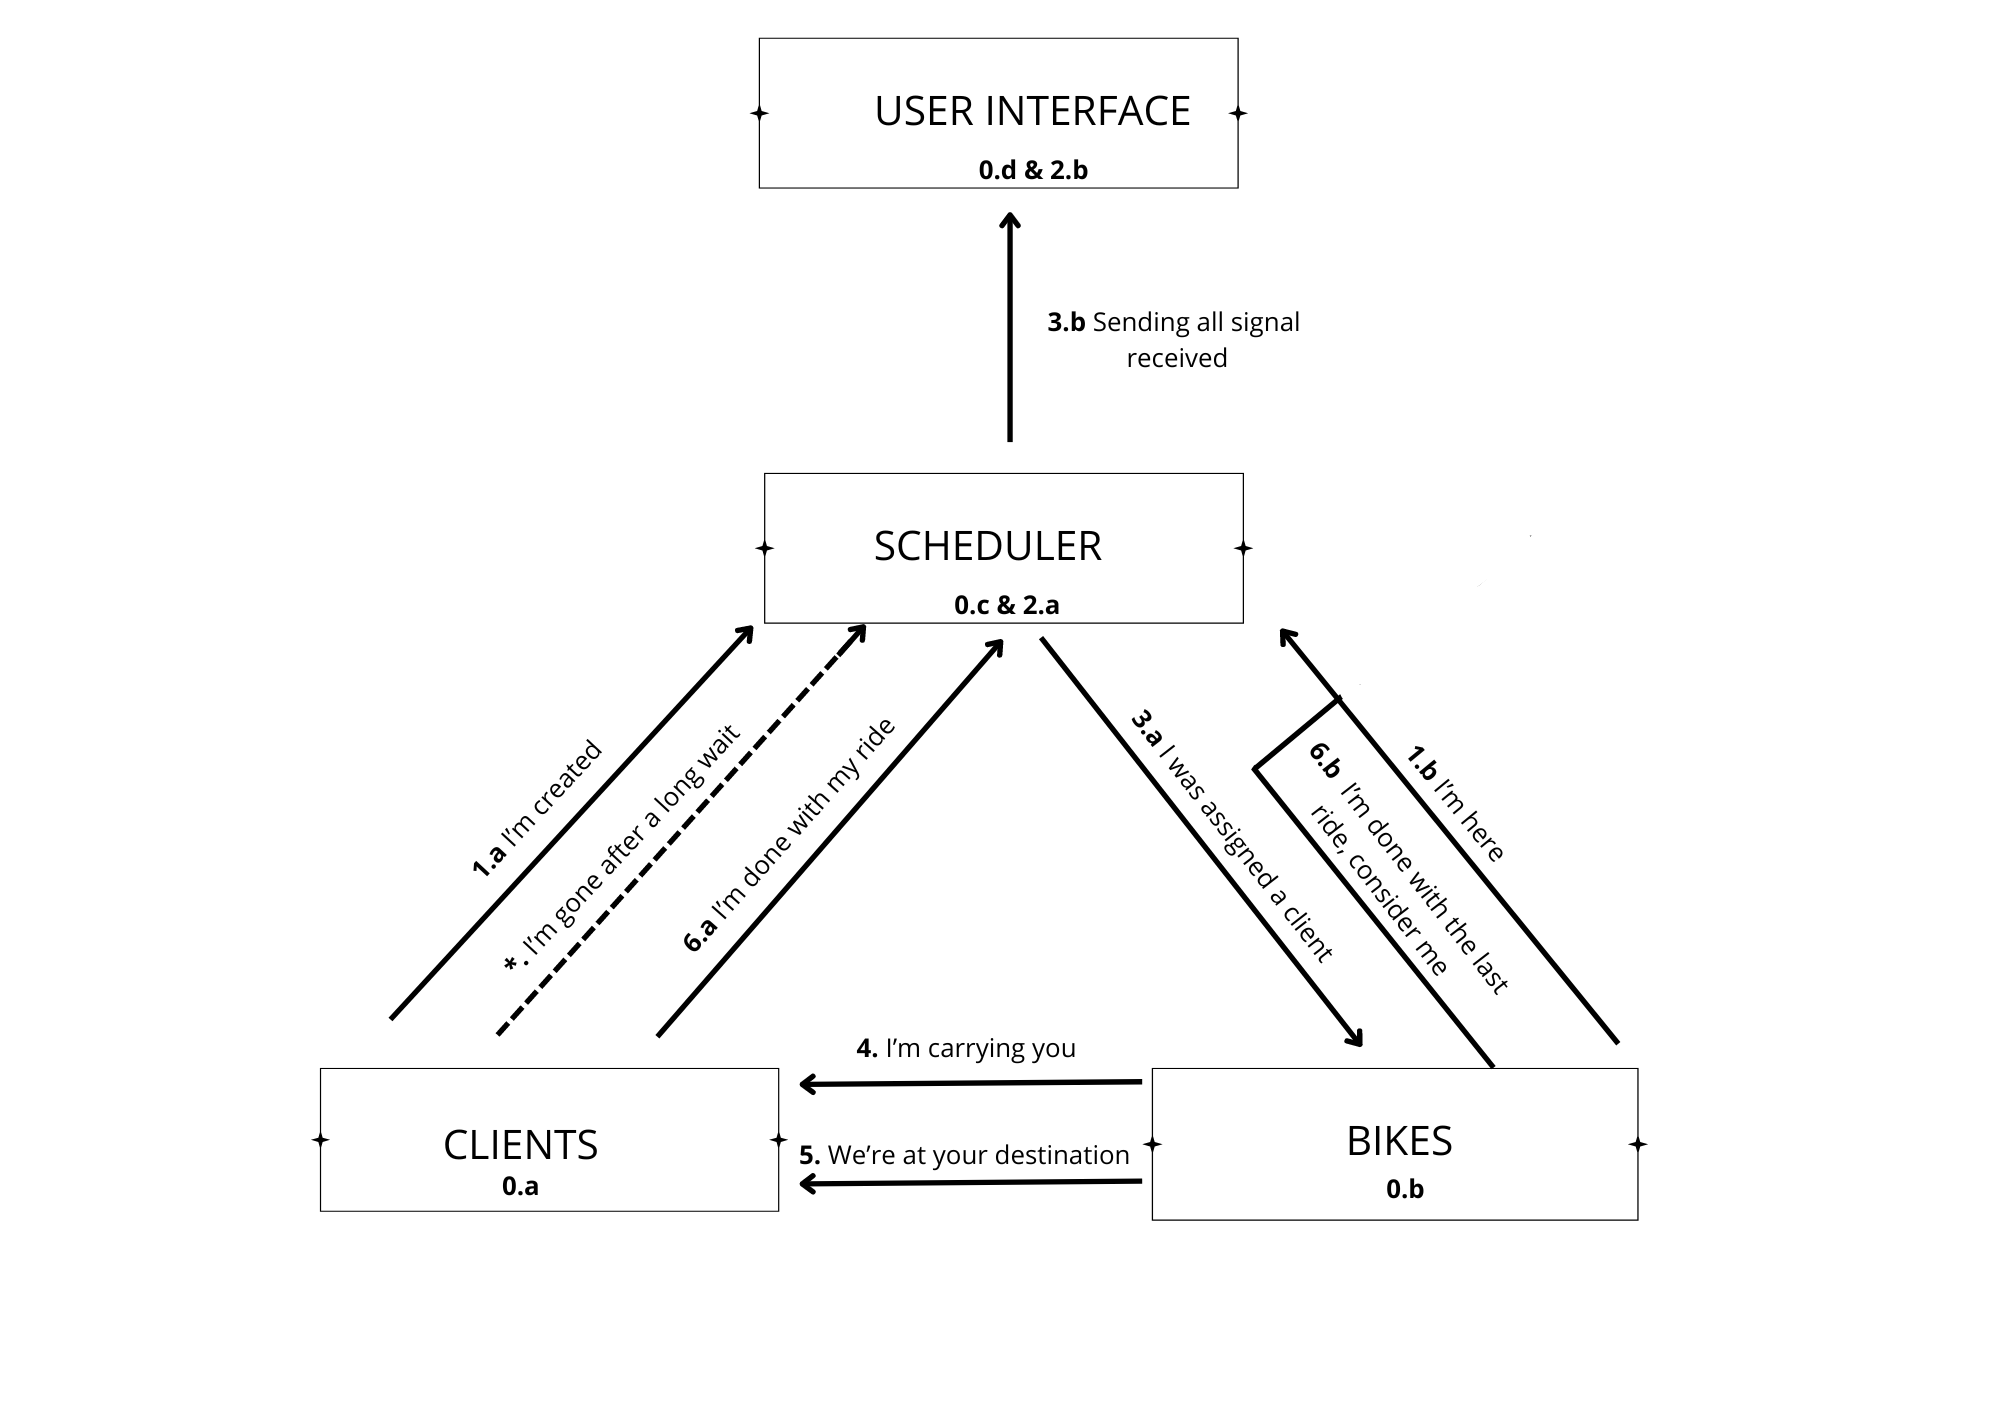
\includegraphics[width=0.7\linewidth]{Sections/Images/fro.png}
%\end{center}




The following figure gives a brief summary of all what has been explicated above.
The numbered sections 0.a, 0.b, 0.c, 0.d, 2.a and 2.b which couldn't be further explained on the figure respectively represent the following:

\begin{enumerate}
  \item \textbf{Step 0.a}:This represents the information generation and the shared memory segment creation.
  \item \textbf{Step 0.b}: This represents the route and the shared memory segment creation.
  \item \textbf{Step 0.c}: This part is concerned with the data initialization and listening mode from the scheduler
  \item \textbf{Step 0.d}: This part is concerned with the initialization of the user interface
  \item \textbf{Step 2.a}: This part is concerned with the different saving of the different bikes and clients information.
  \item \textbf{Step 2.b}: This part is concerned with the the treatment of all the various signals by the user interface.
\end{enumerate}
%-----------------------------------------
\begin{center}
   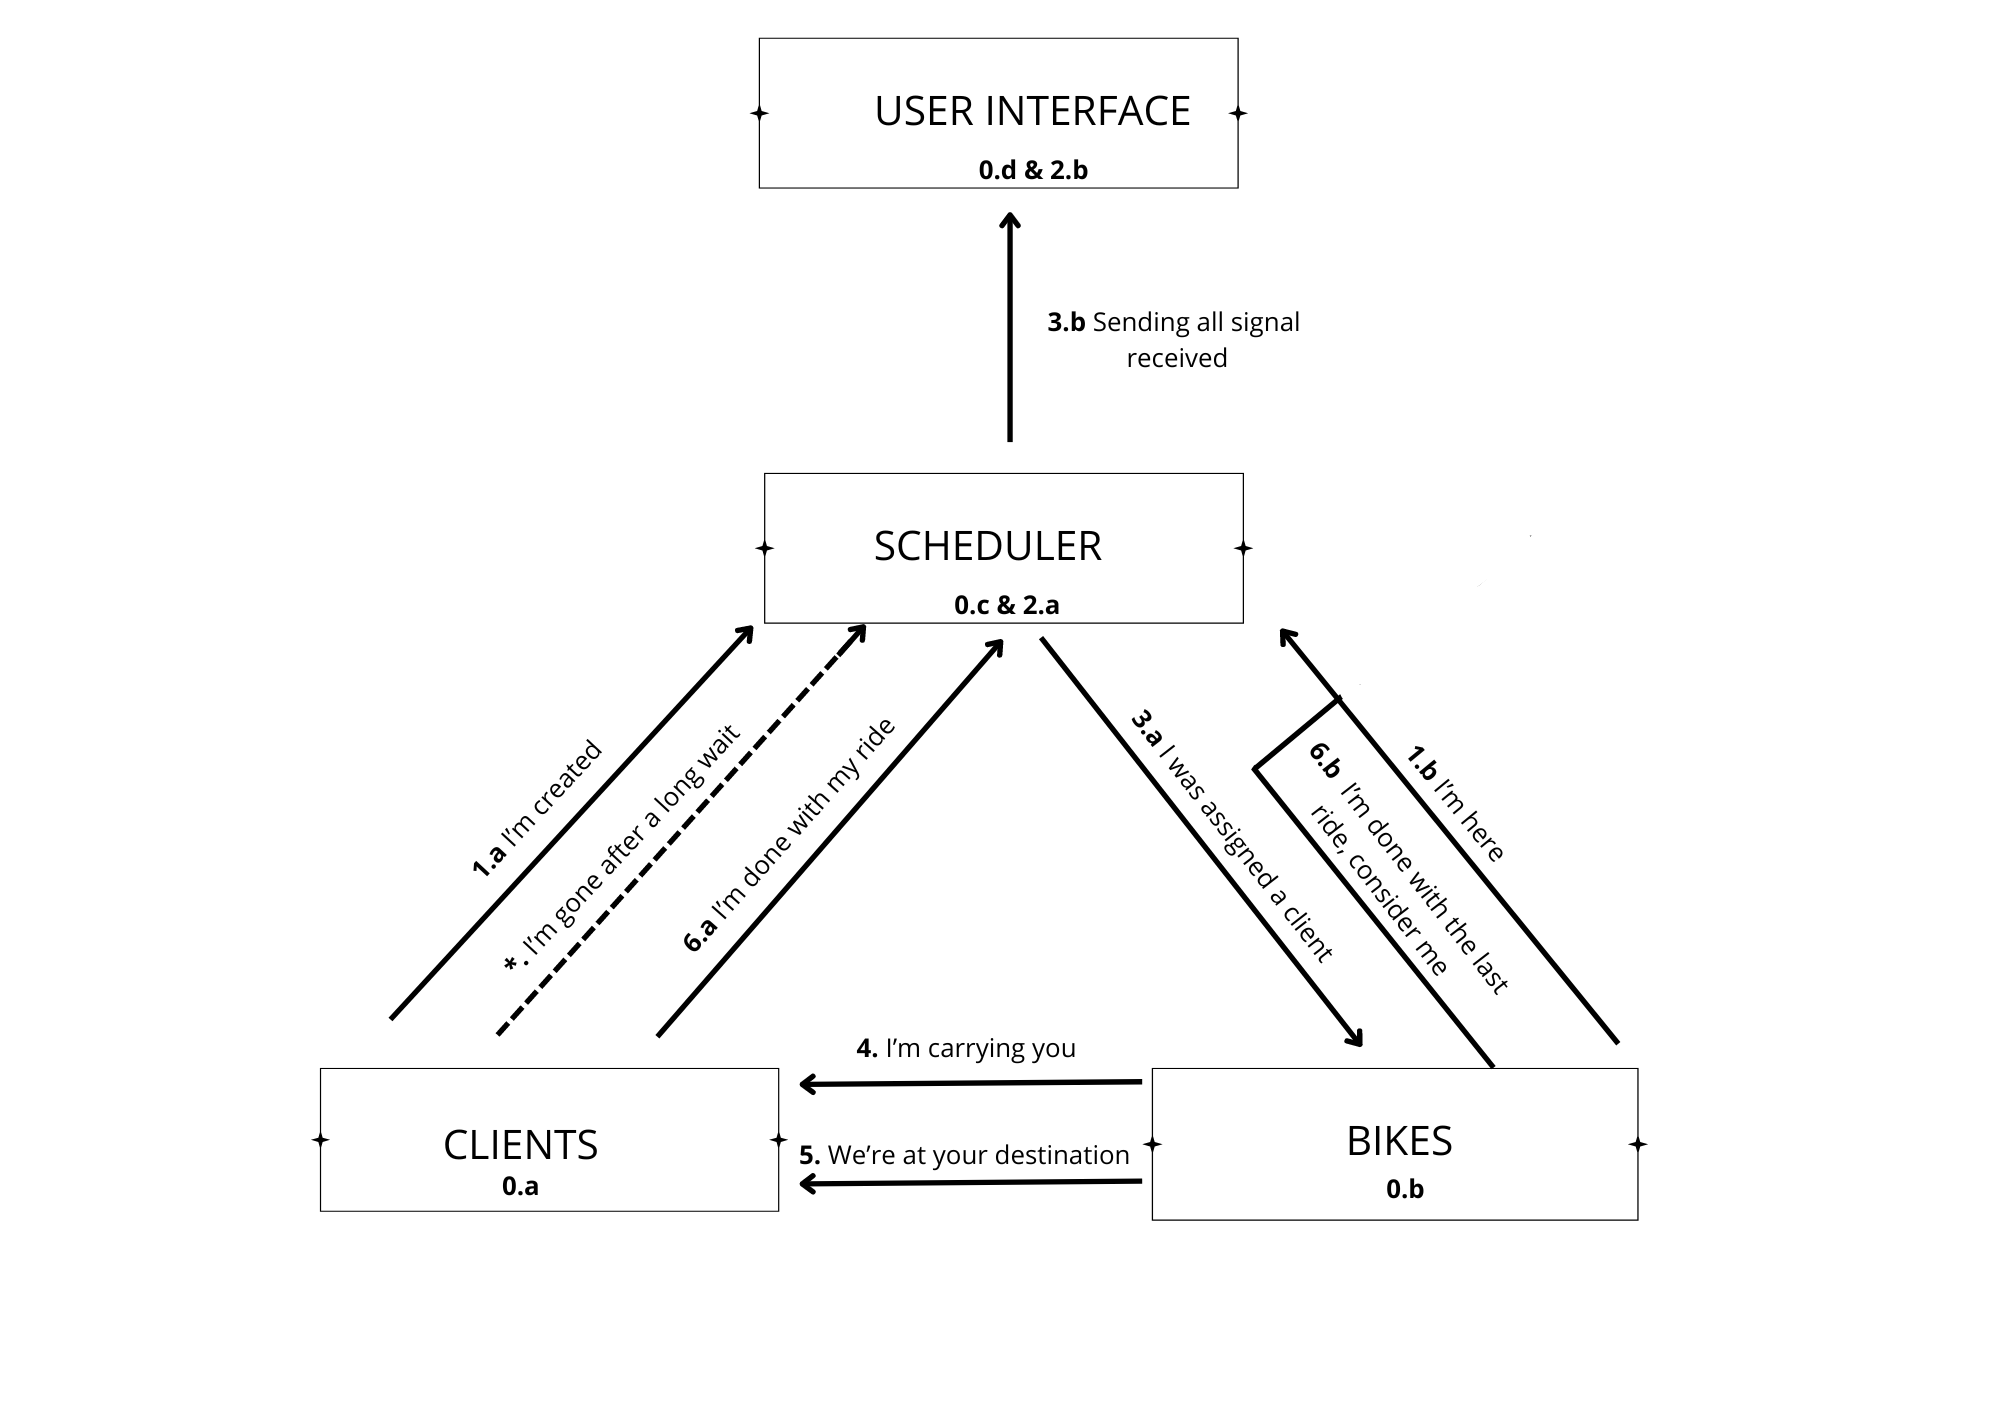
\includegraphics[width=0.7\linewidth]{Sections/Images/fro.png}
\end{center}


\newpage
\subsection{Client and bike}
Graphical clients and motorcycles are simply defined using G-client and G-bike data structures described below.
 \begin{lstlisting}[style=customc, caption={structures for user interface}]
#include <unistd.h>

// 2D point structure
typedef struct Point
{
    float x;
    float y;
}Point;

//client's structure
typedef struct G_client
{
    float radius;
    Point* start;
    Point* dest;
    Point* center;
}G_client;

//bike's structure
typedef struct G_bike
{
    float side;
    Point* start;
    Point* center;
}G_bike;


typedef struct G_quarters 
{
    int id;
    Point *loc;
} G_quarters;


typedef struct G_data
{
    pid_t bike_pid, client_pid;
    int bike_start;
    int client_start, client_dest;

    struct G_data* next;   
}G_data;
\end{lstlisting}
We also define G-quarters structures to describe the graphic area and G-data to link a motorcycle to a client it must go to. This structure will be useful to ensure the simultaneous movement of our motorcycle and client on the interface.
\newpage
\subsection{Scheduler}
The central scheduler operates in this section regarding communication with the background of our project. In fact, it is responsible for informing the interface process about the pairs $(client, motorcycle)$ that need to be moved. It writes this information into a shared memory segment obtained through the \textbf{shmget()} function and sends a signal to the UI using the \textbf{kill()} function. The UI will then read the information from the shared memory segment and use it to simultaneously move both the motorcycle and the client it carries. The information written includes:
\begin{enumerate}
    \item the client's process ID (pid)
    \item the motorcycle's process ID (pid)
    \item the starting and destination points of the client
\end{enumerate}
The UI will then use this data to carry out the movement.

%After we have recovered the user's interface Pid, we will use it to get the scheduler's PId. This is the command to launch this :\\

%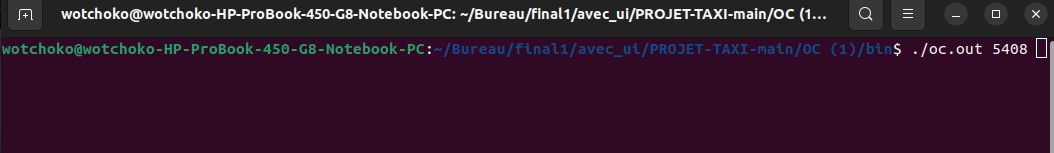
\includegraphics[width=1.0\textwidth]{Sections/Images/oc-out.png}\\

%And this is the result of this command :\\

%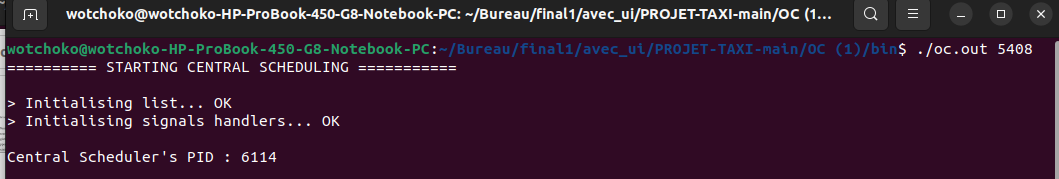
\includegraphics[width=1.0\textwidth]{Sections/Images/oc_pid.png}\\
\newpage
\subsection{UI}
Just as in the scheduler, the UI needs a few data structures to store the information of the clients and motorcycles it needs to display.
\begin{itemize}
    
    \item First, it maps each neighborhood from the backend, stored as an integer, to a graphical neighborhood defined by the G-quar structure mentioned above.
    \item Then, it needs a named list of pairs \texbf{list-t} 
    $(client,moto)$ during display.
\end{itemize}
The UI also needs certain functions to perform its task:
\begin{enumarate}
    \item The function \textbf{init-list()} creates the couple's list $(client,moto)$ for data storage.
    \item The function \textbf{init-quarters-list()} is in charge of creating a correspondence between the quarters back-end and the quarters on the interface and then store it in the quarter-list data structure.
    \item The function \textbf{get-quarter-pos} which allows obtaining the graphical position of a neighborhood based solely on its PID. In fact, it will search the neighborhood list to accomplish this. It returns a graphical point.
    \item A handler \textbf{handle-oc-scheduled} which is used after each scheduling by the scheduler. It allows the UI to read the shared memory segment with the scheduler and retrieve the necessary information to move a pair. $(client,moto)$
    \item The UI also requires specific functions to draw the clients and motorcycles, which we do not consider necessary to list here. Just note that the motorcycles will be represented as squares, while the clients will be represented as circles on the screen.
\end{enumarate}
Here are the function signatures for these functions:
%stp nina regarde uneu ledernier commentaire ans le bloc de code ci-dessous j'arrive pas à bbien formuler.celui du handle%
\newpage
\begin{lstlisting}[style=customc, caption={functions of UI}]
/**
 * @brief initialize bikes and clients tuple list
 * 
 */
void init_list(void)
{
    bikes_n_clients_list = create_list();
}
/** 
 * @brief Function to create many points for display and store them in a list_quarter. 
 * 
 */
void init_quaters_list() 
/**
 * @brief Function to find the coordinates of a quarter based on its ID. 
 * @param id(int) 
 * @return point 
 */
Point* get_quater_pos(int id)
/**
 * @brief handle is used to gather information about couple client-bike which now moves together. 
 * @param signum(int) is a number of signals used to call this handler
 * @param *info(siginfo_t) helps to gather information for the the handle
 * @param *context is of type void 
 */
void handle_oc_scheduled(int signum, siginfo_t *info, void *context)

\end{lstlisting}\newpage